\chapter{\textit{Background}}
Este trabalho aborda, principalmente, dois conceitos importantes. O primeiro diz respeito ao tipo de site que foi investigado e ao qual se tentou propor alguma melhoria de design. O segundo se refere ao ato de coletar algum tipo de informação utilizando, como auxílio, as conexões sociais estabelecidas entre indivíduos. Tal recurso está ligado com a possível melhoria de design estudada durante este trabalho. Portanto, faz-se necessário apresentar neste capítulo: um levantamento em mais detalhes dos significados destes dois conceitos, bem como uma visão geral do que já estava abordado na literatura em relação aos mesmos.

\section{Sites \qa}
Definiu-se para o escopo detste trabalho o conceito de sites \qanospace, que são aqueles os quais são acessados por usuários com o intuito de: realizar perguntas, responder a perguntas ou, ainda, visualizar as discussões geradas por perguntas e os seus respectivos conjuntos de respostas. Os sites \qa são classificados na literatura de duas maneiras distintas: \textit{community} \qa e \textit{social} \qa \cite{gazan2011social}.

\textit{Community} \qa é um termo de uso específico: para um site ser classificado assim, é preciso que haja uma identificação de indicadores formais de comunidade, como usuários se mostrando engajados em divulgá-lo, adotando e expressando uma identidade, etc. \cite{kling2005understanding} Tal classificação é, muitas vezes, feita de forma indiscriminada \cite{rosenbaum2010structuration}.

\textit{Social} \qanospace, de acordo com \cite{gazan2011social}, aparece como um termo mais abragente e se refere aos sites nos quais os respectivos usuários realizam perguntas, respondem a perguntas e avaliam o conteúdo do site enquanto estão interagindo com ele. Apesar de sites deste tipo serem considerados instâncias de comunidades \textit{online} \cite{rosenbaum2010structuration}, o que pode remeter ao conceito de \textit{community} \qanospace, a maior parte dos trabalhos utilizados na elaboração da fundamentação teórica desta pesquisa e, portanto, relevantes neste escopo, opta por utilizar o conceito de \textit{social} \qanospace. Tal opção também foi escolhida durante a elaboração desta dissertação. Portanto, no âmbito desta pesquisa, sites \qa  são, também, definidos como sites do tipo social \qanospace.

Utilizando o \textit{Stack Overflow em Português} (a Figura~\ref{fig:fig1} auxilia nesta ilustração), é possível descrever o modelo de funcionamento de um site \qa (previamente descrito na literatura \cite{furtado2013contributor}):
    \begin{itemize}
        \item Um dado usuário publica alguma pergunta descrevendo um problema;
        \item A pergunta criada é listada no site e visualizada por outros usuários, que podem votar sobre a utilidade ou não da questão, assim como marcá-la como um tópico favorito;
        \item Qualquer usuário pode publicar respostas e comentários que ficam relacionados com a pergunta;
        \item Os demais usuários do site podem visualizar as respostas e comentários, que também podem receber votos;
        \item Comentários neste contexto são utilizados como ferramenta para discussão e esclarecimento entre o usuário que publicou a pergunta (perguntador) e os demais membros do site;
        \item Finalmente, o perguntador pode selecionar uma das respostas como sendo a melhor.
    \end{itemize}
    
Os 3 campos primários de pesquisa em sites \qa presentes na literatura até então são: estudos sobre motivações e comportamentos dos usuários, avaliações da qualidade da informação contida nestes sites e análises de fatores tecnológicos que exercem influência na participação de usuários \cite{shah2009research}.

Este trabalho tem a ver com o campo de avaliações da qualidade da informação, pois houve um esforço para se realizar uma análise quantitativa sobre o efeito do compartilhamento em redes sociais na obtenção ou não de respostas úteis para os autores das perguntas compartilhadas.

    \begin{figure}[H]
        \center
        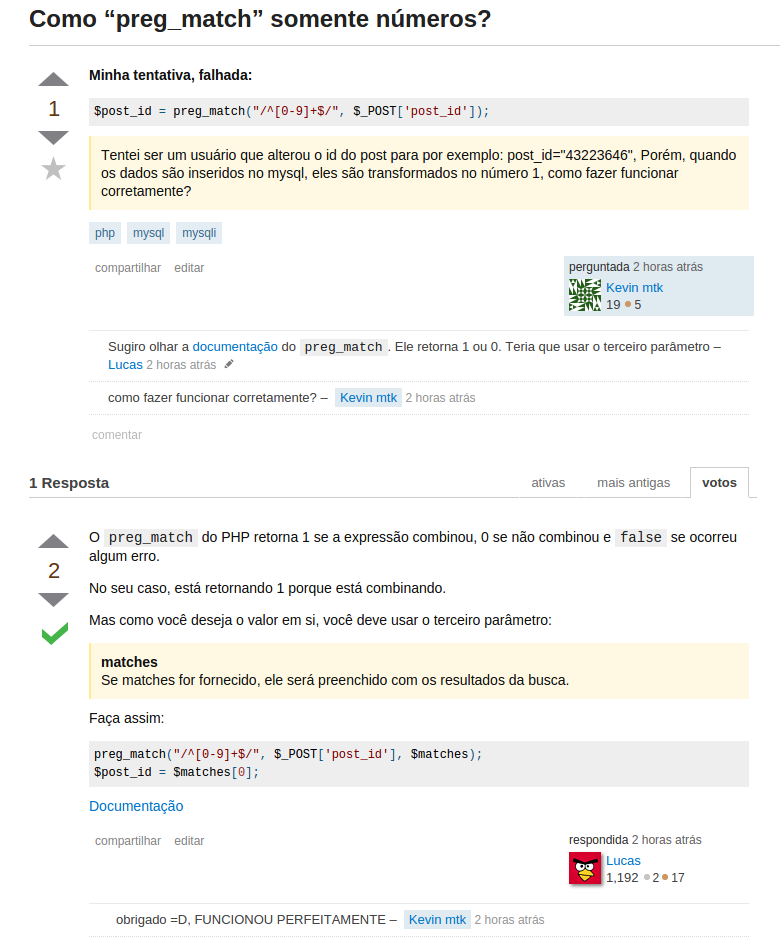
\includegraphics[scale=.6]{./figuras/exemplo-so-pt.png}
        \caption{Página referente a uma questão no \textit{Stack Overflow em Português}.}
        \label{fig:fig1}
    \end{figure}

Existem trabalhos que investigam maneiras de melhorar a qualidade das respostas contidas em sites \qa fomentando-os de alguma forma \cite{harper2008predictors,chen2010knowledge,jeon2010re}. Não foi identificado, na literatura, nenhum esforço para atrair respostas e melhorar a qualidade das mesmas por meio do compartilhamento de perguntas em redes sociais.

No âmbito da avaliação da qualidade do conteúdo em sites \qanospace, aparecem alguns trabalhos interessantes e bastante citados porque analisam o que faz uma resposta receber votos positivos de outros usuários \cite{gazan2006specialists,harper2009facts}. Segundo \cite{gazan2011social}, existem ainda alguns trabalhos importantes e relevantes que discorrem sobre métricas utilizadas para se determinar a qualidade das respostas obtidas em sites \qanospace. De acordo com a literatura, não houve nenhum esforço, até aqui, para saber a influência do ato de compartilhar perguntas de sites \qa em redes sociais na qualidade das respostas obtidas.

É evidente, portanto, que existia na literatura, até a realização desta pesquisa de mestrado, uma oportunidade em aberto de tentar relacionar o compartilhamento em redes sociais com a qualidade e quantidade do conteúdo gerado em sites \qanospace.

% Fica claro que havia, até a realização deste mestrado, uma lacuna na literatura sobre a questão de se compartilhar em redes sociais perguntas oriundas de sites \qanospace. Houve, nesta pesquisa, um esforço para tentar descobrir se compartilhar perguntas de sites \qa nas redes sociais pode ajudar ou não a fomentar tais sites com respostas satisfatórias para os donos das perguntas compartilhadas.

Este estudo aqui presente também está inserido no campo dos estudos sobre motivações e comportamento dos usuários, tendo em vista que abordou a maneira com a qual usuários de sites \qa lidam com a funcionalidade de compartilhar perguntas em redes sociais contida em tais ambientes.

Já foi comprovado anteriormente na literatura que as estruturas de recompensas sociais presentes em sites \qa, como a obtenção de pontos e reputação de acordo com o número de perguntas ou respostas publicadas, formam um ponto crítico para o sucesso e bom funcionamento destes ambientes \cite{shah2008exploring}. Há, inclusive, um trabalho que discorre sobre o efeito destas recompensas na participação dos usuários de tais sites \cite{li2012quantifying}. Entretanto, mais uma vez, não se menciona a questão do compartilhamento de perguntas em redes sociais. É interessante constatar que existe no site \textit{Stack Overflow em Português}, e em vários outros, uma forma de recompensar usuários que compartilham perguntas destes sites em redes sociais (ver Figura~\ref{fig:fig2}).

    \begin{figure}[H]
        \center
        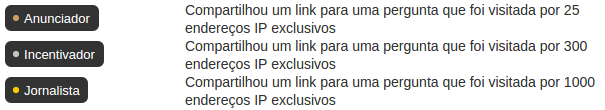
\includegraphics[scale=.6]{./figuras/medalhas-compartilhar-sopt.png}
        \caption{Premiações oferecidas pelo \textit{Stack Overflow em Português} aos usuários que compartilham perguntas deste site em redes sociais.}
        \label{fig:fig2}
    \end{figure}

Trabalhos sobre padrões de participação e de comportamento dos usuários \cite{adamic2008knowledge,furtado2013contributor,bian2008few} foram identificados. Estudou-se os tipos mais comuns de usuários e o que eles faziam de especial (os que apenas perguntavam, os que apenas respondiam, aqueles que só colaboravam de forma específica em certos tipos de postagens, etc.), mas nada foi dito a respeito dos usuários que compartilham perguntas destes sites nas redes sociais.

É natural, então, constatar a lacuna que havia na literatura acerca de trabalhos que relacionam o compartilhamento em redes sociais de perguntas de sites \qa com motivações e comportamento dos usuários, pois nenhum esforço neste sentido foi realizado até então.

\section{\textit{Friendsourcing}}
Tem-se que \textit{crowdsourcing} é um conceito que representa o processo no qual soluções criativas são extraídas de um grupo de indivíduos que se disponibilizam para oferecer algum serviço a partir de uma convocação realizada por parte de quem precisa de tal serviço \cite{brabham2008crowdsourcing}. Por exemplo, imagine um empresa que faça vendas \textit{online} de camisetas cujas estampas são escolhidas por meio de uma competição entre \textit{designers} do mundo todo que estejam querendo mostrar seus trabalhos. Este exemplo existe na prática: é a empresa \textit{Threadless}\footnote{https://www.threadless.com/}.

Usualmente, \textit{crowdsourcing} está relacionado com o recrutamento \textit{online} de indivíduos dispostos a realizar uma tarefa que seria muito trabalhosa ou difícil se fosse feita por uma única pessoa. Em sites que utilizam este conceito, um grande número de usuários incrementam os conteúdos globais destes sites por meio de pequenas contribuições pontuais \cite{Bernstein:2008:PVF:1746259.1746260}. Portanto, é possível afirmar que sites \qa utilizam \textit{crowdsourcing} como forma de fornecer o serviço prometido: encontrar uma resposta para uma dada pergunta realizada por algum usuário.

A partir do que está supracitado, aparece o conceito de \textit{friendsourcing}: uma forma de \textit{crowdsourcing} na qual se visa coletar informação disponível em grupos pequenos e socialmente conectados de maneira precisa \cite{Bernstein:2008:PVF:1746259.1746260}. Tais grupos podem ser, por exemplo, formados por amigos de quem está solicitando o serviço. Um exemplo de \textit{friendsourcing} é alguém perguntar algo aos seus amigos no \textit{Facebook} por meio de uma publicação que esteja visível a todos eles. Existiam, até aqui, trabalhos cujos esforços se basearam em relacionar \textit{friendsourcing} com a realização de perguntas em redes sociais de uma forma diferente do que está nesta dissertação de mestrado. 

Alguns pesquisadores propuseram melhorias na busca em redes sociais por amigos que são capazes de oferecer algum serviço solicitado, como em \cite{Savage:2012:DSQ:2380296.2380321}. Neste trabalho se criou uma ferramenta capaz de auxiliar usuários que desejam requisitar de amigos em redes sociais algum tipo de auxílio, mas que esbarram no problema de se ter uma lista grande de amigos e não saber quem são aqueles com capacidade e interesse em ajudar, o que dificulta a busca por pessoas nesta lista para que esta requisição seja feita de forma direta.

Já em \cite{Brady:2013:IAS:2441776.2441915} se investigou como as pessoas cegas utilizam as redes sociais para tirar dúvidas cotidianas como, por exemplo, perguntar aos amigos quais são as cores das flores presentes em um vaso mostrando uma foto dele. Descobriu-se que, de fato, as redes sociais são muito utilizadas por usuários cegos com tal finalidade. Entretanto, ficou constatato que tais usuários não acham que as redes sociais são os lugares mais apropiados para tal atividade, pois eles demonstraram ter bastante receio em incomodar os amigos e, além disto, não há garantias de que seus amigos irão ajudá-los em tempo hábil.

Além do que já foi discutido nesta seção, também foram identificados na literatura trabalhos nos quais os pesquisadores buscam compreender como se dá o processo de perguntar a amigos em redes sociais. Em \cite{paul2011question} foi conduzida uma pesquisa com o intuito de se determinar como os usuários do \textit{Twitter} se comportam quando querem perguntar algo por meio desta rede social, além de se tentar encontrar os tipos mais comuns de perguntas realizadas neste ambiente.

Seguindo a ideia da pesquisa supracitada, foi encontrado um trabalho bastante relevante na literatura no qual se realizou um estudo mais amplo sobre o comportamento dos usuários das duas redes sociais mais populares da Internet (\textit{Facebook} e \textit{Twitter}) em relação ao ato de realizar perguntas nestes ambientes \cite{morris2010people}. Foram elencados os tipos mais comuns de perguntas realizadas, bem como as motivações dos usuários que perguntam nestas redes sociais, por meio de um questionário respondido por mais de 600 usuários que trabalhavam na empresa \textit{Microsoft}\footnote{http://www.microsoft.com/}.

É importante ressaltar que todos os trabalhos que envolvem \textit{friendsourcing} e o ato de perguntar na Internet são do ponto de vista de quem faz a pergunta. Não havia, até aqui, nenhum trabalho que abordasse a perspectiva de quem utiliza \textit{friendsourcing} nas redes sociais sem, necessariamente, estar querendo beneficiar a si mesmo. Fica constatada, portanto, esta sutil lacuna na literatura que também se abordou durante esta pesquisa de mestrado quando se investigou o uso de \textit{friendsourcing} (compartilhamento de perguntas em redes sociais) como tentativa de fomentar sites \qanospace.

\section{Capital Social}
Capital Social, apesar de apresentar várias definições na literatura, pode ser entendido como um tipo de benefício decorrente da participação em redes ou outras estruturas sociais, sendo utilizado para facilitar novas interações sociais \cite{portes2000social}.

Sendo assim, de acordo com a definição acima, entende-se que, dentro de uma dada rede social, toda e qualquer interação entre indivíduos representará ganho e/ou perda de capital social para alguém. Por exemplo, quando um dado usuário pergunta algo para os seus seguidores no \textit{Twitter} (usuários que acompanham as suas publicações nesta rede), espera-se que aquele que fornecer uma resposta útil ganhará capital social em relação ao usuário autor da pergunta. Por outro lado, também espera-se o seguinte: um certo usuário perde cada vez mais capital social à medida que solicita ajuda a outros em uma dada rede social sem nunca oferecer nada em troca. Portanto, é coerente relacionar o conceito de \textit{friendsourcing} com o de capital social, como foi feito em \cite{rzeszotarski2014estimating}.

Vários trabalhos na literatura tentaram investigar o uso de capital social em redes sociais na Internet. Em \cite{valenzuela2009there} houve um esforço para se determinar se o uso do \textit{Facebook} estava relacionado com o ganho de capital social no cotidiano dos seus usuários por meio de medições de variáveis relacionadas, segundo a sociologia, com capital social, como: participação política, satisfação de vida, engajamento civil, etc. Observou-se que existe uma correlação positiva entre tais fatores.

Destaca-se, também, um trabalho cujo objetivo foi estudar como os diferentes tipos de uso de uma rede social grande e popular como o \textit{Facebook} estão relacionados com o conceito de capital social \cite{Burke:2011:SCF:1978942.1979023}. Neste estudo foi examinado como as seguintes ações estão relacionadas com ganhos e perdas de capital social: comunicação direta entre amigos, \textit{broadcast} de mensagens e leitura de notícias publicadas por terceiros. 

Em \cite{recuero2012economia}, foi identificado um esforço para se relacionar o acesso à informação no \textit{Twitter} com o conceito de capital social. Os resultados deste trabalho sugerem que algumas práticas geram benefícios individuais e coletivos nos quais as replicações de mensagens, ou os \textit{retweets}, atuam como moeda de troca. Há um consenso de que, no \textit{Twitter}, um dos maiores objetivos dos usuários é ter suas mensagens visualizadas pela maior quantidade possível de pessoas dentro da rede. Os pesquisadores discutem que replicar as mensagens de amigos gera ganho de capital social que, posteriormente, pode ser utilizado para replicar novas mensagens, resultando em uma espécie de círculo vicioso.

Atentando para a lacuna existente na literatura, é importante ressaltar que, nesta pesquisa de mestrado, houve um esforço para se estudar como o conceito de capital social está relacionado com o compartilhamento em redes sociais de perguntas oriundas de sites \qanospace. Não foi identificado nehum estudo neste sentido até então. Durante as investigações qualitativas desta pesquisa, procurou-se entender como os usuários enxergavam o capital social relacionado com o compartilhamento de perguntas originalmente publicadas em outros sites e cujos autores muitas vezes não eram eles mesmos.